\documentclass{beamer}
\usetheme{Berkeley}

\usecolortheme{lily}

\title{Beamer Presentation for CSE200}
\subtitle{Using Beamer}
\author{Sheikh Azizul Hakim}
\institute[CSE, BUET]{Department of CSE, BUET}
\date{\today}

\begin{document}

\begin{frame} 
    \maketitle
\end{frame}

\section{Lists \& Stuff}

\begin{frame}{Title of a frame}
    This is our first frame. \pause We want to explore Beamer in this class. 
\end{frame}

\setbeamercovered{transparent}

\begin{frame}{List}

    \begin{itemize}
        \item Point A \pause 
        \item Point B \pause 
        \begin{itemize}
            \item part 1
            \item part 2
        \end{itemize}
        \item Point C
        \item Point D
    \end{itemize}

\end{frame}

\begin{frame}
    \frametitle{More Lists}
    \begin{enumerate}[(I)]
    \item<3-> Point A
    \item<2-> Point B
    \begin{itemize}
    \item<3-> part 1
    \item<4-> part 2
    \end{itemize}
    \item<5-> Point C
    \item<1-2> Point D
    \end{enumerate}
\end{frame}

\begin{frame}{Text Formatting}
    \textbf<2>{Example Text}

    \textit<2-3>{Example Text}

    \textsl<2>{Example Text}

    \textrm<2>{Example Text}

    \textsf<2>{Example Text}

    \textcolor<2>{orange}{Example Text}

    \alert<2>{Example Text}

    \structure<2>{Example Text}
\end{frame}

\begin{frame}{How to use description type lists} 
    \begin{description}
        \item[API] Application Programming Interface
        \item[LAN] Local Area Network
        \item[ASCII] American Standard Code for Information Interchange
    \end{description}
\end{frame} 

\section{Columns \& Table}

\begin{frame}
    \frametitle{Using Columns}
    \begin{columns}
    \column{0.25\textwidth}
    ABCDEFGHIJKL
    \column{0.5\textwidth}
    \begin{figure}
        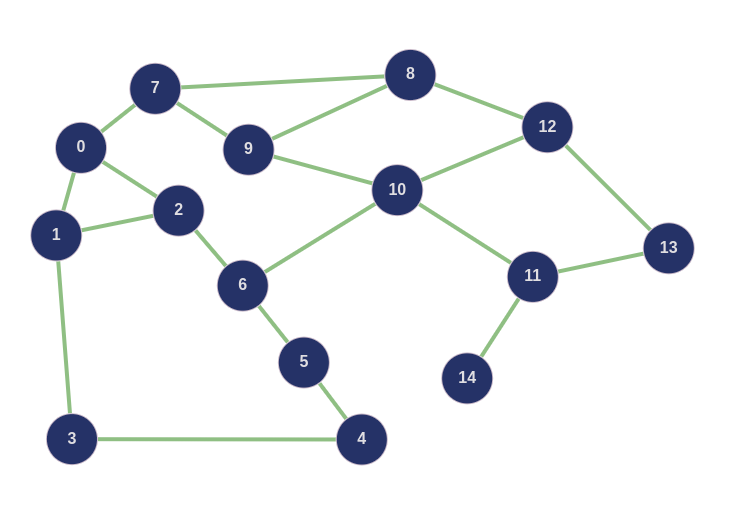
\includegraphics[width=\linewidth]{G_01.png}
    \end{figure}
    \end{columns}
\end{frame}



\begin{frame} 
    \begin{table}
        \begin{tabular}{l | c | c | c | c }
        Competitor Name & Swim & Cycle & Run & Total \\
        \hline \hline
        John T & 13:04 & 24:15 & 18:34 & 55:53 \\ 
        Norman P & 8:00 & 22:45 & 23:02 & 53:47\\
        Alex K & 14:00 & 28:00 & n/a & n/a\\
        Sarah H & 9:22 & 21:10 & 24:03 & 54:35 
        \end{tabular}
        \caption{Triathlon results}
    \end{table}
\end{frame}


\begin{frame}
    \frametitle{Tables}
    \begin{table}
    \begin{tabular}{l | c | c | c | c }
    Competitor Name & Swim & Cycle & Run & Total \\
    \hline \hline
    John T & 13:04 & 24:15 & 18:34 & 55:53 \onslide<2-3> \\ 
    Norman P & 8:00 & 22:45 & 23:02 & 53:47 \onslide<3->\\
    Alex K & 14:00 & 28:00 & n/a & n/a \onslide<4->\\
    Sarah H & 9:22 & 21:10 & 24:03 & 54:35 
    \end{tabular}
    \caption{Triathlon results}
    \end{table}
\end{frame}

\begin{frame}{Example of Blocks}

\begin{block}{BCF24}
    BUET CSE Fest '24 is ongoing. 
\end{block}

\begin{alertblock}{BCF24}
    BUET CSE Fest '24 is ongoing. Hence, students are paying less attention. 
\end{alertblock}

\begin{example}{BCF24 Competitions}
    Competitions of BCF help a lot of students explore many other things on their own.
\end{example}
    
\end{frame}

\begin{frame}{
    Math blocks
}
    \begin{theorem}[Pythagoras] 
    $ a^2 + b^2 = c^2$
    \end{theorem} \pause 
    \begin{corollary}
    $ x + y = y + x  $
    \end{corollary} \pause 
    \begin{proof}
    $\omega +\phi = \epsilon $
    \end{proof}    
\end{frame}

\end{document}